\documentclass[11pt]{article}
\usepackage[margin=1in]{geometry}
\usepackage{graphicx,booktabs,amsmath,hyperref}
\usepackage[T1]{fontenc}
\title{N-gram Hints in Language Model Training}
\author{Vuk Rosi\'c}
\date{}
\begin{document}
\maketitle

\begin{abstract}
An n-gram hint tells a language model which token most often followed the last $n$ tokens in the training data. Hints recently cut the NanoGPT Speedrun record from 39.9 s to 6.7 s. The hints used during training come only from tokens trained in earlier steps, because a large corpus from the start makes the model rely on hints too much. We test this choice on a small character-level transformer trained with Muon. Keeping a token's own occurrence in the counts is the failure to avoid: validation loss goes from 1.89 to 3.53. Removing only that occurrence and dropping half of the hints at random during training gives a loss of 1.80 against 1.89 for hints from earlier steps, and this gap held at about 0.08 across a 15-fold range of model size. The gap grows when the corpus is much larger than the tokens trained (0.37 at 40 times) and disappears when it is 2.5 times larger. We did not reproduce on Shakespeare the reported result that each doubling of the corpus helps more than the last. On web text, leaving out the token's whole page removes the harm at small corpora, and short matches give most of the gain, which shrinks with training. In a made-up language, hints give perfect recall of facts stored in the same words and nothing for other wording, and hints added at the input stop the model from learning two-step comparison and sums. Hints added only at the output, with half dropped, keep the recall and restore that learning. A hint stops mattering once a fact has been stated a few times, and a model that always gets hints memorizes almost nothing itself. When one model trains on web text and these tasks together, hints at all three places block comparison at three model sizes, while output-only hints keep it at the cost of part of the web text gain. The code is public \cite{code}.
\end{abstract}

\section{Introduction}
Language models learn slowly from text they have seen only a few times, and web text is full of passages that repeat only occasionally. Brunborg \cite{brunborg} uses this: during training, idle CPUs build a corpus that records which tokens follow each n-gram. The model receives the most common next token as a hint and learns how much to trust it. The record went from 39.9 s to 6.7 s \cite{pr367}. The blog post reports two things that matter for this paper. A large hint corpus from the start makes the backbone rely on the hints too much, so training uses a small corpus and validation a large one. And each doubling of the corpus cuts the loss more than the last \cite{brunborg}.

The record's code computes training hints in a strictly causal way: a step's hints count only tokens trained in earlier steps \cite{repo}. That has a cost. At validation the model meets hints from a far larger corpus than any it trained with, so it must trust counts it has never seen.

This paper asks one question: if a language model is trained with Muon, can it use hints from the whole corpus from the first step, without the failure the blog post describes, and is that better than hints from earlier steps? We make three contributions.
\begin{enumerate}
\item We show that a token's own occurrence in the counts is enough to break training with a full corpus.
\item We show that removing it, plus random hint dropout, beats causal hints at three model sizes.
\item We measure how the gain depends on the ratio of corpus size to tokens trained.
\item We test what hints help, facts or reasoning, and find that where hints enter the model decides whether it can still learn to reason.
\end{enumerate}

\section{Background}
\paragraph{Muon.} Muon \cite{muon} is an optimizer for the matrices of a network. It keeps momentum, replaces the update with its nearest orthogonal matrix using Newton-Schulz steps, and moves the weights by a fixed step. Its use at large scale is studied in \cite{muonkimi}. Wang et al. \cite{wang} find that Muon learns rare classes better than Adam, which is the same rare-data problem hints address. Embeddings stay on Adam, as is standard.

\paragraph{Memory by lookup.} Engram \cite{engram} adds hashed n-gram embedding tables whose vectors are learned, and Tensorizing Engram \cite{tengram} and Lngram v2 \cite{lngram} extend this line. Hints differ: nothing is learned per n-gram, and the corpus stores only the next tokens. RETRO \cite{retro} retrieves whole text chunks from a very large database.

\paragraph{Leakage.} A count feature that includes the row's own label leaks the label. Target encoding for categorical features has this problem \cite{micci}. CatBoost \cite{catboost} calls the result prediction shift and fixes it with ordered statistics, which use only earlier rows. That is the same idea as causal hints. Leave-one-out statistics are the other common fix. RETRO applies the document-level version: it filters out neighbours from the same document as the training sequence \cite{retro}, so removing the token's own occurrence is not a new idea in retrieval. Our searches found no paper comparing causal and leave-one-out hints for n-gram hints, and none using hint dropout. Dropping an input at random so a model does not rely on it follows dropout \cite{dropout}.

\section{Method}
\paragraph{Model.} We use the Muon lab model \cite{muonlab}: a character-level transformer on Tiny Shakespeare with RoPE, QK-norm, RMSNorm, a SwiGLU MLP, no biases and tied embeddings, with 4 layers and 4 heads. The first 90\% of the text is the training split. Muon trains the hidden matrices with momentum 0.95, and Adam trains the embeddings and norm weights at 0.003. Training has 20 warmup steps and a linear cooldown over the last 30\%.

\paragraph{Hints.} We follow the blog post, with lengths 6, 12 and 24 characters in place of 6, 10 and 20 tokens. For each length the hint is the most common next character. Its count falls into one of 7 buckets and its purity (the share of the n-gram's occurrences followed by that character) into one of 6, giving 126 kinds. Each kind has a learned amount $\sigma$ and a learned vector $\beta$. The hint vector is
\begin{equation}
H_t=\sum_{n}\big(\sigma_{k(n,t)}\,E[\mathrm{hint}_n(t)]+\beta_{k(n,t)}\big),
\end{equation}
where $E$ is the embedding table. We add $H_t$ after the embedding, after layer 2 and before the output head, each with its own learned scale. The hint parameters use Adam at 0.03.

\paragraph{Training hint policies.} Validation always uses the whole training split as its corpus. Training uses one of these:
\begin{itemize}
\item \textbf{None:} no hints.
\item \textbf{Own token kept:} the whole training split, with each token's own occurrence still in the counts.
\item \textbf{Earlier steps:} only tokens trained in earlier steps, as in the record.
\item \textbf{Leave-one-out:} the whole training split with each token's own occurrence removed. If removing it leaves no count, there is no hint, exactly as for an unseen n-gram at validation.
\item \textbf{Leave-one-out with dropout:} the same, and each hint is dropped with probability 0.5.
\end{itemize}
Training streams shuffled, non-overlapping chunks of 65 characters, so a token appears at most once per pass. The default batch is 8 and the default length is 200 steps, or 102K trained tokens. The corpus is 1.0M characters, 10 times the tokens trained. The record's ratio is about 520 times \cite{brunborg}, which a 1 MB text cannot reach.

\paragraph{Measurement.} Each setting was run once at Muon learning rates 0.01, 0.02 and 0.04, and we report the best. Validation uses 96 fixed chunks. Before running, we predicted that own-token-kept would be worst, leave-one-out best, and that hints would make the model worse when they are switched off.

\section{Results}
\subsection{Keeping the token's own occurrence breaks training}
Table~\ref{tab:policy} shows the results at width 64. The predictions held. With the token's own occurrence in the counts, every training n-gram has a match, and a long n-gram usually has only that one occurrence, so the hint is the answer. The model learns to trust hints it will not get at validation. Its loss with hints is 3.53, far worse than 2.16 with no hints at all. Removing that one occurrence brings the loss to 1.84.

\begin{table}[h]\centering
\begin{tabular}{lcc}\toprule
Training hints & Validation, hints on & Validation, hints off\\\midrule
None & -- & 2.165\\
Own token kept & 3.525 & 4.735\\
Earlier steps & 1.890 & 2.307\\
Earlier steps, half dropped & 1.860 & 2.204\\
Leave-one-out & 1.843 & 2.508\\
Leave-one-out, quarter dropped & 1.800 & 2.349\\
\textbf{Leave-one-out, half dropped} & \textbf{1.805} & \textbf{2.256}\\
Leave-one-out, three quarters dropped & 1.807 & 2.206\\\bottomrule
\end{tabular}
\caption{Width 64, 200 steps, batch 8. Best of three learning rates by loss with hints.}\label{tab:policy}
\end{table}

\subsection{Hint dropout removes most of the reliance on hints}
Leave-one-out alone makes the backbone worse when hints are off: 2.508 against 2.165 with no hints. This matches the blog post's report of relying on hints too much. Dropping half of the hints brings this to 2.256 and also lowers the loss with hints from 1.843 to 1.805. Dropping a quarter gives a similar loss with hints (1.800) with a worse backbone (2.349), so we use one half. Dropout also helps earlier-steps hints (1.890 to 1.860), but they stay behind.

\subsection{The gain stays the same as the model grows}
Table~\ref{tab:size} shows a gap between 0.070 and 0.085 across a 15-fold range of parameters. The best learning rate stayed at 0.01 or 0.02 at each size for each policy, so hints did not move Muon's best learning rate in this range.

\begin{table}[h]\centering
\begin{tabular}{rrcccc}\toprule
Width & Parameters & No hints & Earlier steps & Leave-one-out, half dropped & Gap\\\midrule
32 & 56K & 2.317 & 1.938 & 1.858 & 0.081\\
64 & 209K & 2.165 & 1.890 & 1.805 & 0.085\\
128 & 812K & 2.085 & 1.840 & 1.769 & 0.070\\\bottomrule
\end{tabular}
\caption{Validation loss with hints on, 200 steps, batch 8, corpus 10 times the tokens trained.}\label{tab:size}
\end{table}

\subsection{The gain depends on corpus size divided by tokens trained}
Table~\ref{tab:ratio} changes the tokens trained at width 32 with the corpus fixed. The gap is 0.370 at a ratio of 40, 0.081 at 10 and 0 at 2.5, because hints from earlier steps approach the whole corpus as training goes on. At 3200 steps the stream starts a second pass, so hints from earlier steps contain each token's own earlier occurrence. This is the failure from Section 4.1 again: loss rises to 2.533, while leave-one-out reaches 1.603. Causal hints are safe only within one pass.

\begin{table}[h]\centering
\begin{tabular}{rrrcccc}\toprule
Steps & Batch & Ratio & No hints & Earlier steps & Leave-one-out, half dropped & Gap\\\midrule
200 & 2 & 40 & 2.534 & 2.386 & 2.016 & 0.370\\
200 & 8 & 10 & 2.317 & 1.938 & 1.858 & 0.081\\
800 & 8 & 2.5 & 1.956 & 1.676 & 1.676 & 0.000\\
3200 & 8 & 0.6 & 1.755 & 2.533 & 1.603 & 0.930\\\bottomrule
\end{tabular}
\caption{Width 32, hints on. Ratio is corpus size divided by tokens trained. The last row is past one pass over the data.}\label{tab:ratio}
\end{table}

\subsection{Each doubling of the corpus}
We first evaluated models with the first $N$ characters of the training split. The last doubling then gave a gain of 0.237 against 0.09 or less for each earlier one, which looks like the reported acceleration. The last part of the corpus is, however, the text next to the validation split, and the jump disappears when the corpus is sampled evenly. With random 256-character pieces instead, the gains per doubling are 0.040, 0.052, 0.050, 0.060, 0.099, 0.062 and 0.061 for leave-one-out with dropout, and 0.053, 0.055, 0.052, 0.060, 0.073, 0.028 and 0.018 for earlier steps (Figure~\ref{fig:curve}). Neither curve shows gains that rise with each doubling, so we did not reproduce the blog post's result. The share of validation characters with a hint rose from 15\% to 79\%. In the earlier-steps model the loss on hinted characters stops falling after 251K characters (1.74, then 1.75 and 1.77), about 2.5 times its tokens trained, because it never learned how much to trust larger counts. In the leave-one-out model it keeps falling to 1.66.

\begin{figure}[h]\centering
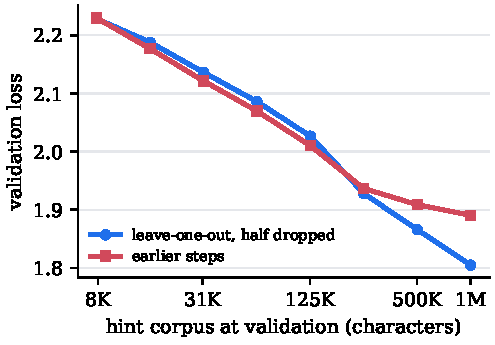
\includegraphics[width=0.62\linewidth]{fig_curve.pdf}
\caption{One final model of each kind evaluated with random subsets of the corpus. Width 64, 200 steps.}\label{fig:curve}
\end{figure}

\section{Web Text}
We repeated the test on FineWeb \cite{brunborg}, using GPT-2 tokens from one 100M-token training shard as the corpus and text from the separate validation shard. Corpus sizes are prefixes of the shard, from 0.78M to 100M tokens. All training chunks lie inside the smallest corpus. The model has width 40, 4 layers, about 1.4M parameters, batch 8 and 90 steps (46K trained tokens) unless stated, with 256 validation chunks. Hints use lengths 6, 10 and 20 tokens unless stated; the longest set adds 2, 3, 4 and 5. Each setting was run once, at the learning rates above unless stated.

\subsection{The hints improve with each doubling on web text}
Before any model is involved, the share of validation tokens where the hint is right grows faster with each doubling (Table~\ref{tab:webhints}). This matches the blog post's report for the hints, unlike our Shakespeare result. We did not check the cause. Near-duplicate pages in both shards are one possibility.

\begin{table}[h]\centering\small
\begin{tabular}{rrrr}\toprule
Corpus & Any hint & Hint right & Added by this doubling\\\midrule
0.78M & 0.42\% & 0.13\% & \\
1.56M & 0.63\% & 0.20\% & 0.07\%\\
3.1M & 0.91\% & 0.28\% & 0.08\%\\
6.25M & 1.30\% & 0.38\% & 0.11\%\\
12.5M & 1.83\% & 0.58\% & 0.19\%\\
25M & 2.65\% & 0.89\% & 0.31\%\\
50M & 3.64\% & 1.35\% & 0.46\%\\
100M & 5.01\% & 2.06\% & 0.71\%\\\bottomrule
\end{tabular}
\caption{Hints of lengths 6, 10 and 20 on 65K validation tokens, with no model. ``Hint right'' is a share of all tokens.}\label{tab:webhints}
\end{table}

\subsection{Leaving out the whole page removes the harm on small corpora}
Validation loss without hints was 7.871. Removing only a token's own occurrence does harm below 25M tokens: hinted tokens score 9.62 at 0.78M and the overall loss is 7.877. Removing every match from the token's own page removes this harm. At 100M the loss is 7.816 with the page left out and no hints dropped, against 7.821 with one occurrence left out and half of the hints dropped. At 50M the page version is 0.003 worse (7.842 against 7.839). With the page left out, dropping half of the hints no longer helps at 100M (7.825). Training hint shares then match validation for 6-grams (4.98\% and 5.01\%) but not for 20-grams (0.77\% and 0.31\%), so same-page repeats do not explain all extra long matches.

\subsection{Short matches give most of the gain, and that gain shrinks with training}
Adding matches of 2, 3, 4 and 5 tokens raises the share of tokens with a hint from 5\% to 92\% and gives by far the largest drop. Loss falls with every doubling of the corpus, from 7.741 at 0.78M to 7.244 at 100M, with gains between 0.045 and 0.107 that rise unevenly. Most of this comes from lengths 2 and 3: at 100M, length 2 alone gives 7.373, and length 4 and longer gives 7.696.

Table~\ref{tab:long} shows what happens with longer training at corpus 100M, with learning rate 0.02. The gain from short matches falls from 0.63 to 0.34 over 16 times more training, because the model learns common next tokens by itself. The gain from lengths 6, 10 and 20 stays between 0.04 and 0.07. The model that uses all seven lengths depends on them: with hints off it scores 7.754 against 6.916 at the longest run.

\begin{table}[h]\centering\small
\begin{tabular}{rrrrr}\toprule
Steps & Tokens trained & No hints & Lengths 6, 10, 20 & All seven lengths\\\midrule
90 & 46K & 7.871 & 7.816 & 7.244\\
360 & 184K & 7.398 & 7.333 & 6.879\\
1440 & 737K & 6.916 & 6.872 & 6.580\\\bottomrule
\end{tabular}
\caption{Validation loss at corpus 100M. Hints leave out the token's own page. The vocabulary grows with the steps (28,359, 39,394 and 46,243 tokens), so compare within a row.}\label{tab:long}
\end{table}

Starting the hints with trust above zero helps a little and did not hurt on small corpora when the own page is left out: at 100M with all seven lengths the loss falls from 7.244 at a starting trust of 0 to 7.197 at 4, the largest value tried, which suggests 90 steps are too few to learn trust.

\section{Facts and Reasoning}
Engram \cite{engram} reports gains on reasoning benchmarks as well as knowledge benchmarks, with learned tables. Wang et al. \cite{wangmem} find that factual questions correlate with n-gram memorization and reasoning tasks with generalization, and Norlund et al. \cite{norlund} find that RETRO's gains largely come from tokens shared with the test data. We found no test of retrieved next-token hints by task kind, so we built a language where the kind of each answer is known.

\paragraph{Setup.} The corpus holds 1.5M lines of made-up text: rare facts stated 3 times each, common facts stated 300 times, sums modulo 10 with 20 of 100 pairs held out, two-step comparisons with fresh names, and reading an answer from the line. Hints use lengths 2, 3, 4 and 6, leave out each token's own occurrence, and enter after the embedding, after layer 2 and before the output head. The model has width 64 and 4 layers, and trains for 5760 steps of 32 lines at learning rate 0.02. We test 1000 new lines per group. Chance is 1\% for facts, about 10\% for sums and 50\% for reading and comparison, where always picking the first name scores that much.

\begin{table}[h]\centering\small
\begin{tabular}{lrrrrrrr}\toprule
Hints & Common & Rare & Other words & Not in table & Held-out sum & Read & Comparison\\\midrule
None & .995 & .009 & .005 & .013 & .492 & .480 & 1.000\\
All 3 places & 1.000 & 1.000 & .010 & .004 & 0 & .502 & .495\\
All 3 places, half dropped & 1.000 & 1.000 & .006 & .012 & 0 & .513 & .495\\
Input only & 1.000 & 1.000 & .006 & .012 & 0 & .513 & .497\\
Length 6 only, all 3 places & 1.000 & 1.000 & .012 & .010 & .730 & .474 & .499\\
Output only & 1.000 & 1.000 & .010 & .003 & 0 & .924 & 1.000\\
\textbf{Output only, half dropped} & \textbf{1.000} & \textbf{1.000} & \textbf{.006} & \textbf{.012} & \textbf{.536} & \textbf{.499} & \textbf{.999}\\\bottomrule
\end{tabular}
\caption{Accuracy at the answer token.}\label{tab:facts}
\end{table}

\paragraph{Results.} Table~\ref{tab:facts} shows that hints take rare facts from chance to 100\% when the test uses the stored words, and give nothing when the words change or the fact is absent. Hints at all three places stop the model from learning comparison (.495 against 1.000) and held-out sums (0 against .492). Hint dropout alone does not fix this. Hints only at the output restore comparison but not sums. Length 6 alone restores sums but not comparison. Output only with half dropped restores both and keeps all recall. As a labelled guess, a hint at the input lets the model skip learning the task, and a confident wrong hint at the output overrides a right answer unless dropout teaches the model to doubt it. Neither arm learned the reading task except output only at .924, which we cannot explain, so it says little.

This does not contradict Engram: its tables are learned, while our hints are retrieved next tokens. A made-up language shows a mechanism, not its size in real models.

\subsection{Web text and reasoning in one model}
Next we trained one model on both languages at once: each step uses 2 web chunks and 32 made-up lines, for 5760 steps. The two languages share no tokens, so one joined hint table gives the same hints as two separate tables. Each language's loss covers only its own tokens, for speed. Web hints use all seven lengths and leave out the token's page, with corpus 100M. We predicted that output-only hints with half dropped would keep at least two thirds of the web text gain, and this failed.

\begin{table}[h]\centering\small
\begin{tabular}{rlrrrr}\toprule
Width & Hints & Web, hints on & Web, hints off & Held-out sum & Comparison\\\midrule
32 & None & -- & 7.132 & .493 & .600\\
32 & All 3 places & 6.824 & 7.846 & 0 & .496\\
32 & Output only, half dropped & 7.095 & 7.107 & .458 & .929\\\midrule
64 & None & -- & 6.991 & .350 & .971\\
64 & All 3 places & 6.714 & 7.637 & .048 & .496\\
64 & Output only & 6.878 & 7.061 & 0 & 1.000\\
64 & Output only, half dropped & 6.971 & 6.991 & .267 & .995\\\midrule
96 & None & -- & 6.956 & .484 & .981\\
96 & All 3 places & 6.677 & 7.602 & 0 & .495\\
96 & Output only & 6.777 & 6.988 & 0 & .995\\
96 & Output only, half dropped & 6.863 & 6.942 & .434 & .996\\\bottomrule
\end{tabular}
\caption{One model trained on web text and the made-up language. Accuracy at the answer token. Rare facts in the table scored 1.000 in every hint row.}\label{tab:mixed}
\end{table}

Table~\ref{tab:mixed} shows a trade-off. Hints at all three places give the largest web text gain, 0.28 to 0.31, and block comparison at all three sizes; with hints off their web loss is 0.65 to 0.71 worse than no hints. Output-only hints keep comparison and keep 41\% of that gain at width 64 and 64\% at width 96. Dropping half restores held-out sums too and leaves the hints-off web loss equal to or better than no hints, but keeps only 12\%, 7\% and 33\% of the gain at widths 32, 64 and 96. The share kept is highest at the largest size, but these are single runs at three sizes spanning 3.2 times the parameters, or 9 times without the embedding table.

\section{How Rare Text Must Be for Hints to Help}
Recall in language models tracks how often a fact appears \cite{kandpal,olmotrace}, and one study reports verbatim recall near 64 exposures at 1B parameters and 16 at 8B \cite{position}, while another finds the entity-frequency effect disappears on some models \cite{memcontext}. For retrieval, kNN-LM papers disagree on whether rare patterns \cite{knnlm} or high-frequency tokens \cite{knnlong} gain most. We found no such split for retrieved next-token hints.

\subsection{A model needs only a few statements of a fact}
Each of 200 facts per group was stated exactly 1, 2, 4 up to 256 times in training, with nothing else in the data. The table holds every fact, so a hint is always right and none are dropped. Table~\ref{tab:rare} shows accuracy without hints. The model reaches 50\% at about 45, 19, 10, 5, 4, 3, 3 and 2 statements at widths 16, 24, 32, 48, 64, 96, 128 and 192, so a wider model needs fewer statements, and the fall flattens above width 96. This agrees in direction with the recall thresholds in \cite{position}, and with a width bound for memorizing facts \cite{geometric}. Going from 2 to 8 layers at width 64 did not move it, so the count does not follow the number of weights. Going from 100 to 400 facts per count moved it from about 4 to 5. With 4 times more training at width 64, every fact stated 4 times as often, the same count gives the same accuracy, so the count matters and not the length of the run. With hints every group scores 100\%. A model trained with hints scores at most 2.5\% with hints off at every count, even at 256 statements: since hints were always right, it memorized almost nothing itself.

\begin{table}[h]\centering\small
\begin{tabular}{lrrrrrr}\toprule
Statements in training & 1 & 2 & 4 & 8 & 16 & 32\\\midrule
Width 16 & .000 & .035 & .005 & .065 & .105 & .260\\
Width 24 & .020 & .025 & .075 & .175 & .395 & .885\\
Width 32 & .030 & .045 & .130 & .380 & .820 & .995\\
Width 48 & .055 & .130 & .350 & .775 & 1.000 & 1.000\\
Width 64 & .060 & .165 & .535 & .870 & .990 & 1.000\\
Width 96 & .120 & .275 & .670 & .935 & 1.000 & 1.000\\
Width 128 & .125 & .310 & .735 & .970 & 1.000 & 1.000\\
Width 192 & .185 & .435 & .775 & .965 & .995 & 1.000\\
Width 64, 2 layers & .070 & .175 & .470 & .850 & .995 & 1.000\\
Width 64, 8 layers & .075 & .175 & .530 & .865 & 1.000 & 1.000\\
Width 64, 400 facts per count & .068 & .145 & .360 & .770 & .965 & 1.000\\
Width 64, 4 times more training & -- & -- & .485 & .885 & .995 & 1.000\\\bottomrule
\end{tabular}
\caption{Accuracy without hints by how many times a fact was stated. Chance is 1\%.}\label{tab:rare}
\end{table}

\subsection{Keeping a model memorizing while it uses hints}
A model that always gets hints stops memorizing, so we tried ways to keep both, at width 64 with the table of Table~\ref{tab:rare} (Table~\ref{tab:mitigate}). Taking the hints away from a random share of tokens works only at a high share: 90\% of tokens without hints matches the model that never saw hints, and 25\% still leaves 70\% accuracy at 256 statements. Stopping hints for the last half of training keeps about half the memorizing, and stopping for only the last quarter also harms the hinted model, whose accuracy falls to 67\% at 256 statements. Hints at the output alone do not help. Two methods keep 100\% with hints and full memorizing where it matters. Training every step on the same batch with and without hints matches the model that never saw hints at every count, for 28\% more clock time. Keeping only text seen under 16 times in the table gives 100\% without hints at 16 statements and above, because there the model gets no hint, and about zero below that, where the table answers. The closest work we found drops privileged inputs in reinforcement learning \cite{pidropout}; R-Drop also runs two passes per batch, but both use the same input \cite{rdrop}. We found no test of these methods on next-token hints.

\begin{table}[h]\centering\small
\begin{tabular}{lrrrrrrr}\toprule
Statements in training & 1 & 4 & 8 & 16 & 32 & 64 & 256\\\midrule
No hints in training & .060 & .535 & .870 & .990 & 1.000 & 1.000 & 1.000\\
Hints always & .000 & .000 & .000 & .000 & .000 & .005 & .005\\
25\% of tokens without hints & .005 & .010 & .015 & .005 & .010 & .140 & .700\\
50\% of tokens without hints & .020 & .010 & .030 & .060 & .285 & .915 & 1.000\\
75\% of tokens without hints & .045 & .235 & .555 & .960 & 1.000 & 1.000 & 1.000\\
90\% of tokens without hints & .070 & .425 & .785 & .985 & 1.000 & 1.000 & 1.000\\
Share without hints rises 0 to 100\% & .010 & .065 & .195 & .505 & .870 & .995 & 1.000\\
No hints in last half & .045 & .225 & .515 & .865 & .995 & 1.000 & 1.000\\
No hints in last quarter & .005 & .040 & .055 & .175 & .375 & .765 & 1.000\\
Hints at output only & .020 & .000 & .010 & .000 & .010 & .030 & .010\\
Output only, 50\% without hints & .050 & .250 & .490 & .815 & 1.000 & 1.000 & 1.000\\
Every step with and without hints & .065 & .475 & .890 & .985 & 1.000 & 1.000 & 1.000\\
Table keeps text seen under 16 times & .015 & .025 & .000 & 1.000 & 1.000 & 1.000 & 1.000\\\bottomrule
\end{tabular}
\caption{Accuracy with hints off, width 64, one run each. With hints on, every row scores at least 99\% except no hints in the last quarter.}\label{tab:mitigate}
\end{table}

\subsection{Only training with and without hints survives web text and reasoning}
We repeated the best methods in the joint model of Table~\ref{tab:mixed} at width 64 (Table~\ref{tab:fix}). Training every step with and without hints keeps 96\% of the web text gain with hints on, and with hints off it beats the model that never saw hints by 0.039. With hints off it also recovers sums and comparison, so one trained model can answer both ways. It costs 47\% more clock time than hints alone. It has two limits. With hints on, reasoning stays blocked, and a common fact reaches only 7\% with hints off against 78\% without hints, unlike in the facts-only test. A table of rare text fails here: it loses most or all of the web text gain and comparison stays at chance, for reasons we did not establish. Dropping hints from 75\% of tokens keeps 44\% of the gain.

\begin{table}[h]\centering\small
\begin{tabular}{lrrrrrr}\toprule
Training & Web on & Web off & Sum on/off & Comparison on/off & Fact off & Gain\\\midrule
No hints & -- & 6.991 & .350 & .971 & .780 & --\\
All three places & 6.714 & 7.637 & .048/.000 & .496/.014 & .012 & 100\%\\
\textbf{With and without hints} & \textbf{6.726} & \textbf{6.952} & .040/.403 & .500/.960 & .070 & 96\%\\
Output only, with and without & 6.924 & 6.980 & .270/.270 & .979/.979 & .036 & 24\%\\
75\% of tokens without hints & 6.868 & 6.991 & .222/.222 & .914/.774 & .270 & 44\%\\
Table under 16 times & 7.010 & 7.077 & .581/.581 & .495/.505 & 1.000 & 0\%\\
Table under 64 times & 6.933 & 7.132 & .349/.349 & .499/.488 & 1.000 & 21\%\\
Under 16, with and without & 6.985 & 6.972 & .148/.148 & .543/.971 & 1.000 & 2\%\\\bottomrule
\end{tabular}
\caption{One model on web text and the made-up language, width 64, 5760 steps, one run each. Hints enter at all three places unless named. Gain is the share of the 0.277 web text gain of hints at all three places. Fact off is a common fact with hints off.}\label{tab:fix}
\end{table}

\subsection{On web text the gain sits on text the model itself has not seen}
We split the gain of 0.357 at 1440 steps over 65K validation tokens (Table~\ref{tab:split}). Gain per token rises with match length, from 0.22 at length 2 to 3.98 at length 20, where the hint is right 92\% of the time, but lengths 2 to 4 hold 72\% of the gain because they cover far more tokens. By how many times the match was seen in the corpus the gain is nearly flat, from 0.29 to 0.53 per token, and it is highest for matches seen once. True next tokens seen 1K to 100K times hold 74\% of the gain on 46\% of tokens, and tokens seen over 100K times hold 14\% on 42\%, which disagrees with \cite{knnlong}. Hints that are right, on 18\% of tokens, give 125\% of the gain, and wrong hints take back 20\%. These models sit at a loss near 6.9, so this describes early training only.

The count above comes from the 100M token table, but the model trained on only 737K tokens, 1/135 of that, so text seen 16 times in the table is usually text the model never saw. Table~\ref{tab:modelseen} counts what the model itself saw. Of tokens with a full context in their chunk, 79\% of the gain sits on contexts the model never saw. Gain per token falls from 0.42 at zero sightings to 0.14 at 16 to 63 and to about zero at 64 or more, which agrees with the facts test.

\begin{table}[h]\centering\small
\begin{tabular}{lrrr}\toprule
Group & Share of tokens & Share of gain & Gain per token\\\midrule
No match & 8\% & $-4$\% & $-0.17$\\
Longest match 2 to 4 & 80\% & 72\% & 0.32\\
Longest match 5 & 7\% & 11\% & 0.56\\
Longest match 6 & 4\% & 12\% & 1.05\\
Longest match 10 & 0.6\% & 5\% & 3.16\\
Longest match 20 & 0.3\% & 3\% & 3.98\\\midrule
Match seen once & 19\% & 28\% & 0.53\\
Match seen 2 to 15 times & 35\% & 39\% & 0.40\\
Match seen 16 or more times & 38\% & 37\% & 0.35\\\bottomrule
\end{tabular}
\caption{Web text gain of hints of all seven lengths. The two blocks split the same tokens.}\label{tab:split}
\end{table}

\begin{table}[h]\centering\small
\begin{tabular}{lrrr}\toprule
Times the model saw the context & Share of tokens & Share of gain & Gain per token\\\midrule
0 & 67.2\% & 79.2\% & 0.421\\
1 & 7.9\% & 8.3\% & 0.377\\
2 to 3 & 4.7\% & 5.1\% & 0.393\\
4 to 15 & 5.0\% & 3.7\% & 0.265\\
16 to 63 & 2.3\% & 0.9\% & 0.138\\
64 or more & 1.5\% & $-0.1$\% & $-0.026$\\\bottomrule
\end{tabular}
\caption{Web text gain split by sightings in the model's own 737K training tokens, for the 88.6\% of tokens whose longest match fits inside their chunk.}\label{tab:modelseen}
\end{table}

\section{Limits}
\begin{itemize}
\item The made-up language tests use one training length, so they have no length check. Facts runs took about 190 s, joint runs 537 to 1267 s, and rarity runs 43 to 311 s, over our usual 10 s limit. We did not split the web text gain by token kind.
\item The web text models stop at a loss far above real models, so they do not show what hints do for a trained model. The 360-step and 1440-step runs took 59 to 214 s, and web runs at 90 steps took up to 11.3 s, over our usual 10 s limit.
\item Shakespeare is not web text. It has no crawled duplicates, its tokens are characters, and 6-grams match 79\% of validation but carry little information. The blog post's rising returns may need exact duplicates at long n-grams, so this does not contradict it.
\item Each setting was run once, and learning rates were picked on the same validation chunks used for reporting, for every arm alike.
\item The 800-step, 3200-step and width-128 runs took 11 to 97 s, over our usual 10 s limit. The batch of 53 runs that included them took 3 minutes 18 seconds on 8 cores.
\item The ratio in Table~\ref{tab:ratio} changes together with tokens trained, so we did not measure a fixed ratio at longer training.
\item Our model trains no more than 1.6M characters, far from a real run, and we did not test the corpus sizes at which a hint table stops fitting in memory. In a real run, leave-one-out needs the full corpus before training starts, or a table large enough to subtract one count per lookup.
\end{itemize}

\section{Open Questions}
Each question below can be tested without the others.
\begin{enumerate}
\item If a GPT-2-sized model is trained with Muon on web text, does adding n-gram hints from the training data lower validation loss compared with the same model trained without hints?
\item If a model much larger than GPT-2 is trained on web text, do n-gram hints still lower validation loss by a useful amount compared with the same model without hints?
\item If a model is trained on web text with hints, does each doubling of the hint corpus lower validation loss by more than the doubling before it, even after near-duplicate documents are removed from the training data?
\item If a model is trained on web text with a hint corpus about 500 times larger than the tokens it trains on, does removing each token's own occurrence and dropping half of the hints give lower validation loss than using hints from earlier steps only?
\item If a model keeps using a hint table when it answers, how much of the loss gain is lost when the table is cut from 352 GiB to 1\% of that size by keeping only the most common n-grams?
\item If a model is trained with hints, does it repeat training text word for word more often than the same model trained without hints, both with the hints on and with them off?
\item If two models are tested on rare facts that appear only a few times in the training data, does the model with hints answer more of them correctly than the model without hints?
\item If a model is tested on text that shares no documents with the training data, do hints still lower its loss compared with the same model without hints?
\item If the ratio of hint corpus size to tokens trained is held fixed while training gets longer, does the gain from removing each token's own occurrence and dropping half of the hints stay the same?
\end{enumerate}

\section{Planned Experiments}
The small models above have not learned common next tokens, so we plan these experiments next.
\begin{enumerate}
\item If the n-gram table predicts each validation token on its own, with no model, is its loss lower than the 7.24 of the small model that uses hints?
\item If the model receives the table's counts for all next tokens as additions to its output scores, instead of the embedding of the most common next token, is its validation loss lower?
\item If the vocabulary is cut to the 2,000 most common tokens plus one token for all others, so that each step is faster, does a model given the same time reach a lower validation loss, measured against the same model without hints at that vocabulary?
\item If a model trains far beyond 16 times longer than our first web text run, does the validation loss gain from short matches disappear?
\item If a model with hints at the output is made much larger, does the share of the web text loss gain it keeps, compared with hints at all three places, keep rising?
\item If the web text loss gain is split by token kind, do names and numbers gain more than other tokens only when the match is long?
\item If a model is trained with and without hints on every step, can a learned gate stop hints from blocking reasoning while they stay on?
\item If a hint table drops n-grams that the model itself has already seen often, instead of those common in the corpus, how much of the web text gain is kept at a much lower loss than we reached?
\end{enumerate}

\section{Conclusion}
For hints from a full corpus, remove each token's own occurrence (on web text, its whole page), and drop half of the hints during training. If the model must also learn to reason, add hints only at the output: in a made-up language this kept perfect recall of stored facts and restored comparison, which hints at all three places blocked at every size we tried. This costs part of the web text gain, so it is a trade-off, and dropping half of the hints restores sums too at a larger cost. In a small Muon-trained model this beat hints from earlier steps by about 0.08 at three sizes, and by more when the corpus was far larger than the tokens trained. If a run makes more than one pass, causal hints need the same removal. To stop hints from replacing the model's own learning, train every step both with and without hints: in our joint test this kept 96\% of the web text gain and reasoning with hints off, for 47\% more clock time, though not recall of common facts and not reasoning with hints on. As a labelled guess, the size of this gain at the record's ratio of about 520 could be larger than in our 40 times case, but web text may behave differently, so it must be tested on FineWeb.

\begin{thebibliography}{99}\small
\bibitem{brunborg} H. Brunborg. N-gram hinted language modeling: NanoGPT Speedrun in 6.7s. \url{https://brunborg.com/n-gram-hinted-lm}, 2026.
\bibitem{pr367} Track 1: Retrieval-augmented n-gram hints. Pull request 367, \url{https://github.com/KellerJordan/modded-nanogpt/pull/367}.
\bibitem{repo} H. Brunborg. n-gram-hinted-lm, file \texttt{old\_records/online\_hints.py}. \url{https://github.com/hermabr/n-gram-hinted-lm}.
\bibitem{muon} K. Jordan. Muon: an optimizer for hidden layers in neural networks. \url{https://kellerjordan.github.io/posts/muon/}, 2024.
\bibitem{muonkimi} Muon is scalable for LLM training. arXiv:2502.16982, 2025.
\bibitem{wang} Wang et al. Muon outperforms Adam in tail-end associative memory learning. arXiv:2509.26030, 2025.
\bibitem{engram} Conditional memory via scalable lookup: a new axis of sparsity for large language models. arXiv:2601.07372, 2026.
\bibitem{tengram} Tensorizing Engram: sharing latents across n-gram embeddings is beneficial in LLMs. arXiv:2606.08347, 2026.
\bibitem{lngram} Lngram v2: latent n-gram memory with interpretable discrete representations. arXiv:2609.03426, 2026.
\bibitem{retro} Improving language models by retrieving from trillions of tokens. arXiv:2112.04426, 2021.
\bibitem{micci} D. Micci-Barreca. A preprocessing scheme for high-cardinality categorical attributes in classification and prediction problems. SIGKDD Explorations, 2001.
\bibitem{catboost} L. Prokhorenkova et al. CatBoost: unbiased boosting with categorical features. NeurIPS, 2018.
\bibitem{dropout} N. Srivastava et al. Dropout: a simple way to prevent neural networks from overfitting. JMLR, 2014.
\bibitem{muonlab} V. Rosi\'c. Muon lab. \url{https://github.com/vukrosic/muon-lab}, 2026.
\bibitem{kandpal} N. Kandpal et al. Large language models struggle to learn long-tail knowledge. ICML, 2023.
\bibitem{olmotrace} Tracing multilingual factual knowledge acquisition in pretraining. arXiv:2505.14824, 2025.
\bibitem{position} Positional fragility in LLMs: how offset effects reshape our understanding of memorization risks. arXiv:2505.13171, 2025.
\bibitem{memcontext} Memory vs. context? Influential factors of factual recall in language models. arXiv:2609.24238, 2026.
\bibitem{knnlm} Generalization through memorization: nearest neighbor language models. arXiv:1911.00172, 2019.
\bibitem{knnlong} Long-tail crisis in nearest neighbor language models. arXiv:2503.22426, 2025.
\bibitem{wangmem} X. Wang et al. Generalization v.s. memorization: tracing language models' capabilities back to pretraining data. ICLR, 2025. arXiv:2407.14985.
\bibitem{norlund} T. Norlund et al. On the generalization ability of retrieval-enhanced transformers. arXiv:2302.12128, 2023.
\bibitem{code} V. Rosi\'c. ngram-hints-llm: code for this paper. \url{https://github.com/vukrosic/ngram-hints-llm}, 2026.
\bibitem{geometric} S. Ravfogel, G. Yehudai et al. Geometric Factual Recall in Transformers. arXiv:2605.12426.
\bibitem{pidropout} Privileged Information Dropout in Reinforcement Learning. arXiv:2005.09220.
\bibitem{rdrop} X. Liang, L. Wu et al. R-Drop: Regularized Dropout for Neural Networks. NeurIPS 2021.
\end{thebibliography}
\end{document}
